Designet af robotten for dette projekt er yderst vigtigt; det er grundstenen i projektet, og uden en velfungerende robot (og specifikt kontrol af denne), vil det blive yderst svært at løse problemstillingen for projektet tilfredsstillende.
Dette afsnit fokuserer på hvordan vi er kommet frem til designet af den endelige robot, samt hvilke særlige problemstillinger der ligger til grund for designet.

\subsection{Design overvejelser}\label{robot:design}
Designet af robotten har været en del af læringsprocessen for hvordan man bygger en robot af \lego NXT komponenterne, hvorfor design processen kan ses som en iterativ process, hvor designet er blevet radikalt ændret for hver iteration, indtil et tilfredsstillende resultat er opnået.


\paragraph{Erfaringer fra tidligere designs} 
Der blev konstrueret flere forslag til en robot inden det endelige resultat. 
I dette afsnit vil det blive gennemgået hvilke erfaringer disse initierende designs gav.


\begin{itemize}
\item Hvis NXT enheden fungerede som base med alle andre komponenter monteret på, vanskeliggjorde det at finde en god placering af robottens ultrasoniske sensor.

\item Hvis sensoren monteres i 1:1 forhold mellem motoren der roterer den, er der alt for store usikkerheder når sensoren skal roteres x-antal grader (ofte mere end 5\degree).
Disse usikkerheder er et resultat af den manglende præcisionen forbundet med styringen af motoren samt slid af dens interne komponenter, hvilke vores test også beskriver i \cref{sensorer:motorer}.
\end{itemize}

\paragraph{Design krav}
Disse to design ledte frem til følgende krav til det endelige design af robotten:

\begin{itemize}
\item Den ultrasoniske sensor skal kunne styres med  minimum 1\degree~nøjagtighed, med en foreslået gearing på 1:4.
\item Sensoren(e) skal kunne foretage en 360\degree~måling.
\item Sekundært indføres der en gearing af hjulene for bedre styring af robotten (nedgearing for højere moment).
\item Mere stabil opbygning for at mindske generelle usikkerheder (bl.a. sidder hjulene bedre fast på basen).
\end{itemize} 


\subsection{Endeligt design}
Udgangspunktet for det endelige design er baseret på ovenstående design krav sammen med andre idéer der tilsammen skal øge præcisionen af robotten og gøre den nemmere at styre.

\begin{figure}
\centering
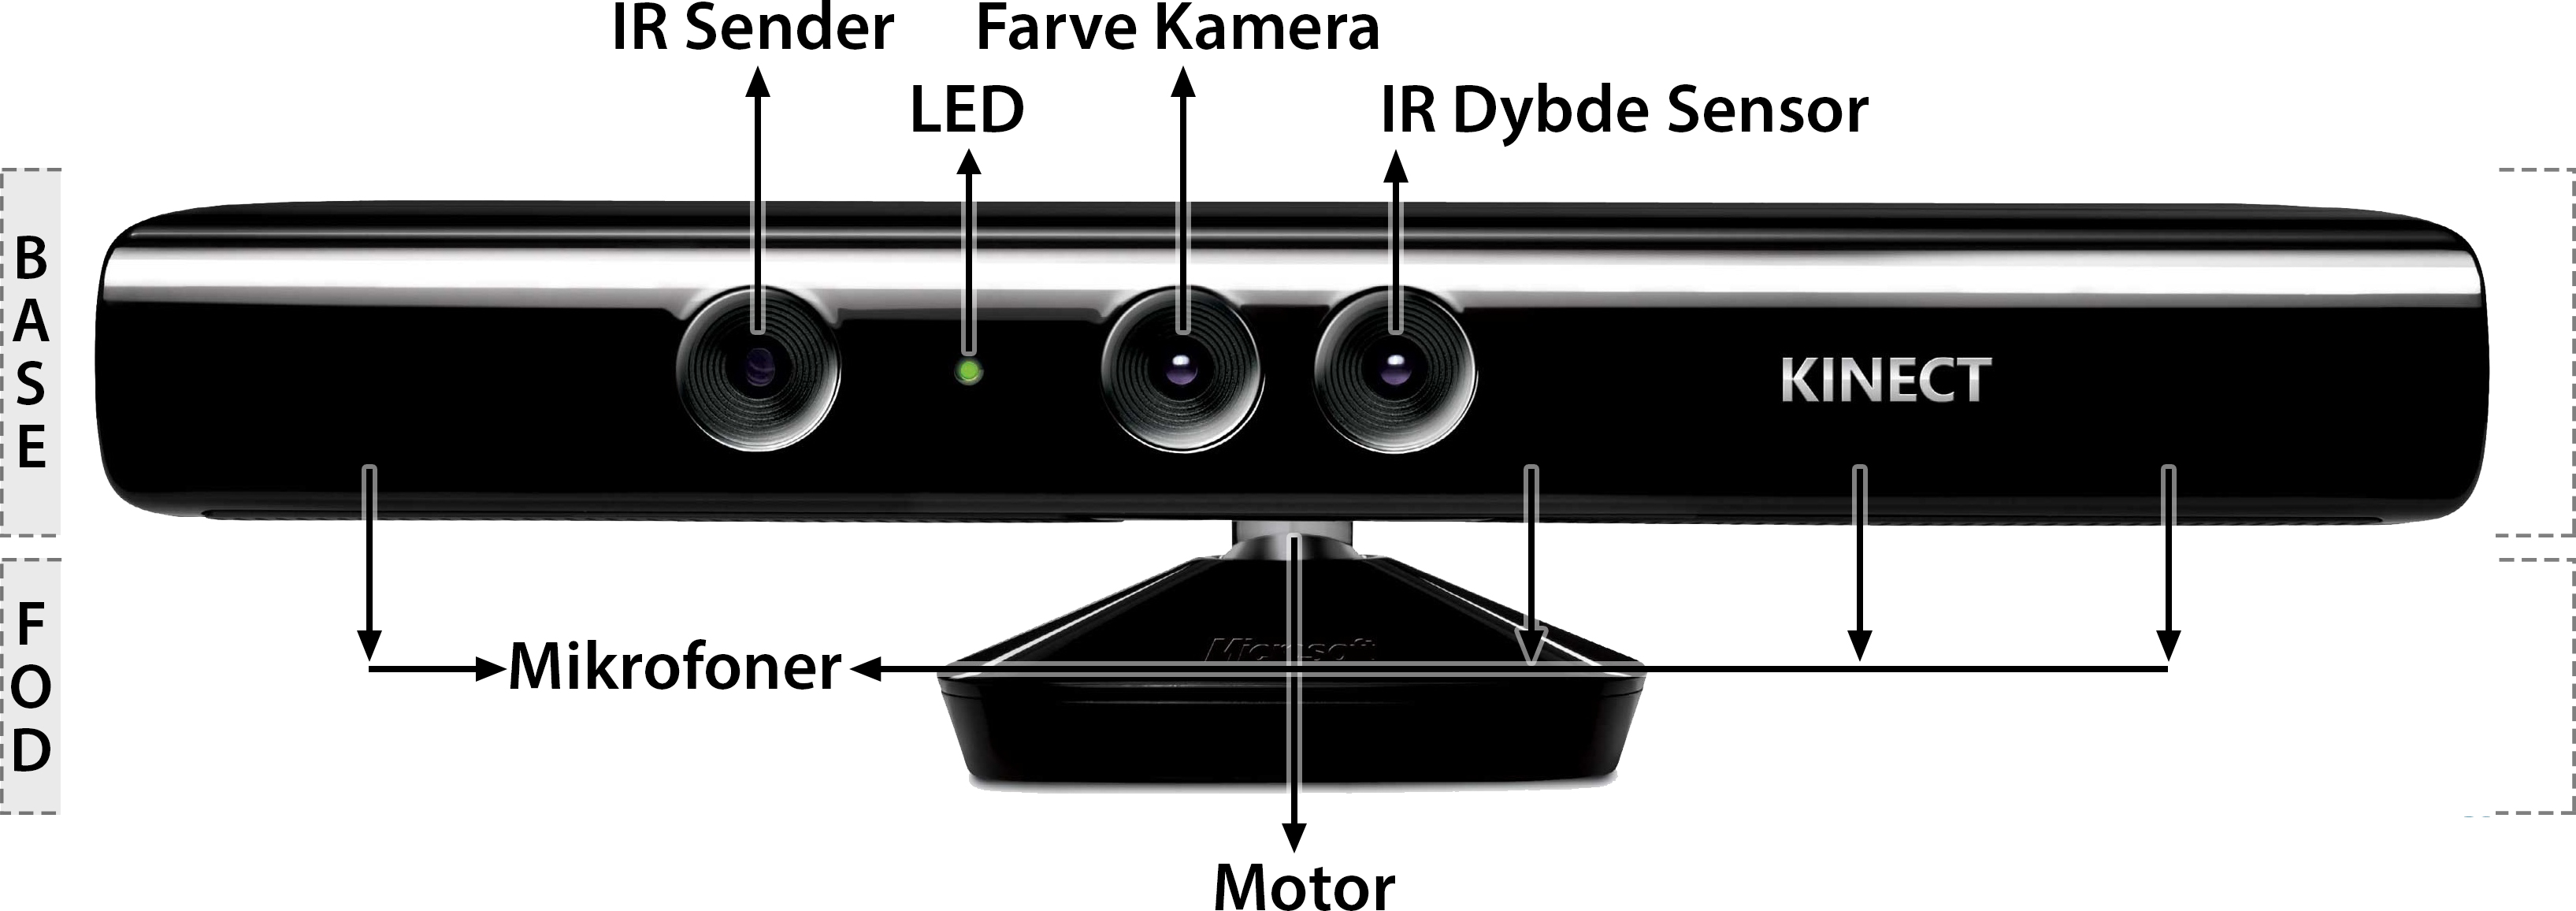
\includegraphics[width=0.5\textwidth]{kinect/kinect}
\caption{Endelige design af vores robot.\thilemann{Insæt billede af robot her, beskriv dimensioner}}
\label{robot:opbygning}
\end{figure}

\subsubsection{Komponenters placering}

Den vigtigste faktor når robotten bygges er placeringen af de primære komponenter, såsom de ultrasoniske sensorer der skal foretage afstandsmålinger og motoren der skal skabe fremdrift.

\paragraph{Kroppen}
Er det som 'holder robotten sammen'.
Det er en central komponent som er bygget op omkring motorene som styrer henholdsvis hjulene og rotation af sensorerne.
Desuden er NXT enheden også en central del af denne konstruktion.
Placeringen af denne er primært i forhold til funktionelle behov, da der på fronten er knapper til at tænde/slukke og vælge indstillinger med.
Der er også taget hensyn til adgang til dens porte for tilslutning af motor, sensor samt opladning.

Vigtigt for basen er højden i forhold til armen hvorpå sensorerne er monteret; for at disse skal kunne se i alle retninger er det essentielt at basens relative højde er så lav som muligt i forhold til de ultrasoniske sensorer, således den ikke er en faktor når de ser bagud i retningen af basen. 

\paragraph{Fremdrift}
Robotten er konstrueret med et \textit{aktivt} hjulsæt der både giver fremdrift og styring.
Denne funktionalitet opnås ved at hvert hjul (på hver side af robotten) har sin egen motor, således der kan angives både positiv og negativ fremdrift uafhængigt af hvert hjul.
Dette design gør det muligt at rotere robotten omkring sin egen akse for maksimal mobilitet -- selv på et begrænset område.
Foruden det ene hjulsæt er der bagerst på robotten monteret et 'baghjul', hvis eneste funktion er at balancere/stabilisere robotten.
Valget af et hjul til at udføre en sådan funktion er ret begrænset i \lego, hvorfor valget faldt på et 'slæbehjul' med en masse ruller der gør det muligt for hjulet at rotere i alle retninger.

På de to første design af robotten var der monteret to store (Ø81,6mm x 15mm) hjul direkte på motorene.
Denne løsning fungerede fint i forhold til højden af basen (og det faktum at robotten stod så godt som vandret), men da gummiet på disse hjul er meget fleksible i forhold til sideværts bevægelse (når robotten roterer), blev det vurderet at det vil give for store usikkerheder ved beregningen af rotationen, samt det faktum at der er en sandsynlighed for at gummiet kan vrides af fælgen med det resultat at robotten ikke kan køre videre.
\stefan{Skete det, eller er det noget vi bare siger? Hvad er ``en sandsynlighed''?}
Derfor er der valgt et lavere og bredere hjul som er meget mere stabilt (Ø56mm x 26mm).
Med dette valg samt den højere friktion (større kontaktflade med underlaget), er det valgt at geare motorene der styrer hjulene, hvilket er beskrevet i \cref{robot:gearing}.

\paragraph{Sensorer}
Den egentlige funktion af robotten er at tage afstandsmålinger til objekter indenfor sensorernes rækkevidde.
Placeringen af disse er derfor ikke kritisk, da de højst vil give en forskydelse af konstant faktor relativ til robottens midte fra deres placering i fronten.
Vigtigere er at der er 360\degree~udsyn når de roterer og at robotten ikke skaber interferens, hvilket er løst ved at montere sensorerne højere end resten af robotten. 
\stefan{Skaber robotten interferens?}


\thilemann{Der bør nok i ovenstående 3 paragraffer laves henvisninger til det kommende billede af robotten}



